% Options for packages loaded elsewhere
\PassOptionsToPackage{unicode}{hyperref}
\PassOptionsToPackage{hyphens}{url}
%
\documentclass[
]{book}
\title{Học xác suất thống kê qua phần mềm R}
\author{Tan-Duc Nguyen}
\date{2022-05-13}

\usepackage{amsmath,amssymb}
\usepackage{lmodern}
\usepackage{iftex}
\ifPDFTeX
  \usepackage[T1]{fontenc}
  \usepackage[utf8]{inputenc}
  \usepackage{textcomp} % provide euro and other symbols
\else % if luatex or xetex
  \usepackage{unicode-math}
  \defaultfontfeatures{Scale=MatchLowercase}
  \defaultfontfeatures[\rmfamily]{Ligatures=TeX,Scale=1}
\fi
% Use upquote if available, for straight quotes in verbatim environments
\IfFileExists{upquote.sty}{\usepackage{upquote}}{}
\IfFileExists{microtype.sty}{% use microtype if available
  \usepackage[]{microtype}
  \UseMicrotypeSet[protrusion]{basicmath} % disable protrusion for tt fonts
}{}
\makeatletter
\@ifundefined{KOMAClassName}{% if non-KOMA class
  \IfFileExists{parskip.sty}{%
    \usepackage{parskip}
  }{% else
    \setlength{\parindent}{0pt}
    \setlength{\parskip}{6pt plus 2pt minus 1pt}}
}{% if KOMA class
  \KOMAoptions{parskip=half}}
\makeatother
\usepackage{xcolor}
\IfFileExists{xurl.sty}{\usepackage{xurl}}{} % add URL line breaks if available
\IfFileExists{bookmark.sty}{\usepackage{bookmark}}{\usepackage{hyperref}}
\hypersetup{
  pdftitle={Học xác suất thống kê qua phần mềm R},
  pdfauthor={Tan-Duc Nguyen},
  hidelinks,
  pdfcreator={LaTeX via pandoc}}
\urlstyle{same} % disable monospaced font for URLs
\usepackage{color}
\usepackage{fancyvrb}
\newcommand{\VerbBar}{|}
\newcommand{\VERB}{\Verb[commandchars=\\\{\}]}
\DefineVerbatimEnvironment{Highlighting}{Verbatim}{commandchars=\\\{\}}
% Add ',fontsize=\small' for more characters per line
\usepackage{framed}
\definecolor{shadecolor}{RGB}{248,248,248}
\newenvironment{Shaded}{\begin{snugshade}}{\end{snugshade}}
\newcommand{\AlertTok}[1]{\textcolor[rgb]{0.94,0.16,0.16}{#1}}
\newcommand{\AnnotationTok}[1]{\textcolor[rgb]{0.56,0.35,0.01}{\textbf{\textit{#1}}}}
\newcommand{\AttributeTok}[1]{\textcolor[rgb]{0.77,0.63,0.00}{#1}}
\newcommand{\BaseNTok}[1]{\textcolor[rgb]{0.00,0.00,0.81}{#1}}
\newcommand{\BuiltInTok}[1]{#1}
\newcommand{\CharTok}[1]{\textcolor[rgb]{0.31,0.60,0.02}{#1}}
\newcommand{\CommentTok}[1]{\textcolor[rgb]{0.56,0.35,0.01}{\textit{#1}}}
\newcommand{\CommentVarTok}[1]{\textcolor[rgb]{0.56,0.35,0.01}{\textbf{\textit{#1}}}}
\newcommand{\ConstantTok}[1]{\textcolor[rgb]{0.00,0.00,0.00}{#1}}
\newcommand{\ControlFlowTok}[1]{\textcolor[rgb]{0.13,0.29,0.53}{\textbf{#1}}}
\newcommand{\DataTypeTok}[1]{\textcolor[rgb]{0.13,0.29,0.53}{#1}}
\newcommand{\DecValTok}[1]{\textcolor[rgb]{0.00,0.00,0.81}{#1}}
\newcommand{\DocumentationTok}[1]{\textcolor[rgb]{0.56,0.35,0.01}{\textbf{\textit{#1}}}}
\newcommand{\ErrorTok}[1]{\textcolor[rgb]{0.64,0.00,0.00}{\textbf{#1}}}
\newcommand{\ExtensionTok}[1]{#1}
\newcommand{\FloatTok}[1]{\textcolor[rgb]{0.00,0.00,0.81}{#1}}
\newcommand{\FunctionTok}[1]{\textcolor[rgb]{0.00,0.00,0.00}{#1}}
\newcommand{\ImportTok}[1]{#1}
\newcommand{\InformationTok}[1]{\textcolor[rgb]{0.56,0.35,0.01}{\textbf{\textit{#1}}}}
\newcommand{\KeywordTok}[1]{\textcolor[rgb]{0.13,0.29,0.53}{\textbf{#1}}}
\newcommand{\NormalTok}[1]{#1}
\newcommand{\OperatorTok}[1]{\textcolor[rgb]{0.81,0.36,0.00}{\textbf{#1}}}
\newcommand{\OtherTok}[1]{\textcolor[rgb]{0.56,0.35,0.01}{#1}}
\newcommand{\PreprocessorTok}[1]{\textcolor[rgb]{0.56,0.35,0.01}{\textit{#1}}}
\newcommand{\RegionMarkerTok}[1]{#1}
\newcommand{\SpecialCharTok}[1]{\textcolor[rgb]{0.00,0.00,0.00}{#1}}
\newcommand{\SpecialStringTok}[1]{\textcolor[rgb]{0.31,0.60,0.02}{#1}}
\newcommand{\StringTok}[1]{\textcolor[rgb]{0.31,0.60,0.02}{#1}}
\newcommand{\VariableTok}[1]{\textcolor[rgb]{0.00,0.00,0.00}{#1}}
\newcommand{\VerbatimStringTok}[1]{\textcolor[rgb]{0.31,0.60,0.02}{#1}}
\newcommand{\WarningTok}[1]{\textcolor[rgb]{0.56,0.35,0.01}{\textbf{\textit{#1}}}}
\usepackage{longtable,booktabs,array}
\usepackage{calc} % for calculating minipage widths
% Correct order of tables after \paragraph or \subparagraph
\usepackage{etoolbox}
\makeatletter
\patchcmd\longtable{\par}{\if@noskipsec\mbox{}\fi\par}{}{}
\makeatother
% Allow footnotes in longtable head/foot
\IfFileExists{footnotehyper.sty}{\usepackage{footnotehyper}}{\usepackage{footnote}}
\makesavenoteenv{longtable}
\usepackage{graphicx}
\makeatletter
\def\maxwidth{\ifdim\Gin@nat@width>\linewidth\linewidth\else\Gin@nat@width\fi}
\def\maxheight{\ifdim\Gin@nat@height>\textheight\textheight\else\Gin@nat@height\fi}
\makeatother
% Scale images if necessary, so that they will not overflow the page
% margins by default, and it is still possible to overwrite the defaults
% using explicit options in \includegraphics[width, height, ...]{}
\setkeys{Gin}{width=\maxwidth,height=\maxheight,keepaspectratio}
% Set default figure placement to htbp
\makeatletter
\def\fps@figure{htbp}
\makeatother
\setlength{\emergencystretch}{3em} % prevent overfull lines
\providecommand{\tightlist}{%
  \setlength{\itemsep}{0pt}\setlength{\parskip}{0pt}}
\setcounter{secnumdepth}{5}
\usepackage{booktabs}
\ifLuaTeX
  \usepackage{selnolig}  % disable illegal ligatures
\fi
\usepackage[]{natbib}
\bibliographystyle{plainnat}

\usepackage{amsthm}
\newtheorem{theorem}{Theorem}[chapter]
\newtheorem{lemma}{Lemma}[chapter]
\newtheorem{corollary}{Corollary}[chapter]
\newtheorem{proposition}{Proposition}[chapter]
\newtheorem{conjecture}{Conjecture}[chapter]
\theoremstyle{definition}
\newtheorem{definition}{Definition}[chapter]
\theoremstyle{definition}
\newtheorem{example}{Example}[chapter]
\theoremstyle{definition}
\newtheorem{exercise}{Exercise}[chapter]
\theoremstyle{definition}
\newtheorem{hypothesis}{Hypothesis}[chapter]
\theoremstyle{remark}
\newtheorem*{remark}{Remark}
\newtheorem*{solution}{Solution}
\begin{document}
\maketitle

{
\setcounter{tocdepth}{1}
\tableofcontents
}
\hypertarget{stat-learning}{%
\chapter{Stat learning}\label{stat-learning}}


\includegraphics[width=1\textwidth,height=\textheight]{images/Quotefancy-237580-3840x2160.jpg}
\href{mailto:tanduc307@gmail.com}{\nolinkurl{tanduc307@gmail.com}}

\hypertarget{how-to-use-tools}{%
\chapter{How to use tools}\label{how-to-use-tools}}

\hypertarget{tux1ea1o-thux1b0-mux1ee5c-luxe0m-viux1ec7c}{%
\section{Tạo thư mục làm việc}\label{tux1ea1o-thux1b0-mux1ee5c-luxe0m-viux1ec7c}}

Khi sử dụng Rstudio thì nên tạo thư mục project để toàn bộ files sẽ nằm trong đó.

Cách thực hiện xem ở đây \url{https://alexd106.github.io/intro2R/howto.html\#rstudio_proj-vid}

Lợi thế là trong folder project này, ta có thể tạo các folder con như images, data, tables, \ldots{} để thuận tiện lưu riêng từng loại dữ liệu. {[}hiện tại làm sao để cấu hình cho hình ảnh nó tự động lưu theo từng folder thì chưa biết cách, thấy có package `here' mà không biết cách dùng).

Lưu ý là khi dùng bookdown để render books thì tên của heading là ghi tiếng Anh cho lành, vì nếu ghi tiếng Việt thì nó render bị lỗi unicode.

RStudio Projects from intro 2R on Vimeo.

\hypertarget{chuxe8n-huxecnh-ux1ea3nh}{%
\section{Chèn hình ảnh}\label{chuxe8n-huxecnh-ux1ea3nh}}

Có các cách chèn hình khi sử dụng Rstudio như sau:

• Chuyển qua chế độ Visual rồi insert hình ảnh. Sau đó hình ảnh sẽ được lưu trong folder \_book/images khi render bằng knitr.

• Nếu gõ theo kiểu source code thì dùng đoạn mã sau
\texttt{\textasciigrave{}\textasciigrave{}\textasciigrave{}\ \{r\ echo=TRUE,\ paged.print=FALSE,\ out.width="30\%"\}\ knitr::include\_graphics("images/cover.jpg")\ \textasciigrave{}\textasciigrave{}\textasciigrave{}}

\begin{Shaded}
\begin{Highlighting}[]
\NormalTok{knitr}\SpecialCharTok{::}\FunctionTok{include\_graphics}\NormalTok{(}\StringTok{"images/cover.jpg"}\NormalTok{)}
\end{Highlighting}
\end{Shaded}


\includegraphics[width=0.3\linewidth]{images/cover}

• Nếu copy và paste từ trên Internet thì dùng add-on \texttt{imageclipr} \href{https://github.com/Toniiiio/imageclipr}{\textless https://github.com/Toniiiio/imageclipr\textgreater{}}. Hình ảnh sẽ lưu mặc định trong working directory.

• Nếu copy và paste hình ảnh theo kiểu thủ công thì hình ảnh mặc định sẽ lưu ở \texttt{C:/Users/tandu/AppData/Local/RStudio/tmp/paste-B717C571.png} như vậy thì khi xuất bản online sẽ không thấy. Do đó phải đưa hình ảnh vào trong thư mục project (theo kiểu thủ công) hoặc dùng add-on \texttt{imageclipr} theo kiểu trực tiếp trong Rstudio (nhưng ở dạng Rmarkdown, còn Rmarkdown visual thì bị lỗi).

\hypertarget{chuxe8n-video}{%
\section{Chèn video}\label{chuxe8n-video}}

Sử dụng link này \url{https://video-to-markdown.marcomontalbano.com/} (theo kiểu click vào hình rồi direct qua source để play video)

Chèn từ Youtube, sử dụng code embed rồi paste vào.

\texttt{\textless{}iframe\ width="560"\ height="315"\ src="https://www.youtube.com/embed/RLxV3T2b524"\ title="YouTube\ video\ player"\ frameborder="0"\ allow="accelerometer;\ autoplay;\ clipboard-write;\ encrypted-media;\ gyroscope;\ picture-in-picture"\ allowfullscreen\textgreater{}\textless{}/iframe\textgreater{}}

Tuy nhiên video sẽ không tự động resize theo khung cửa sổ

Nên dùng code này để video tự động resize. Chiều rộng và cao 100\% có nghĩa là theo khung cửa sổ chứ không phải theo kích thước gốc của video.

\texttt{\textless{}div\ style="position:relative;padding-bottom:56.25\%;"\textgreater{}\ \ \textless{}iframe\ style="width:100\%;height:100\%;position:absolute;left:0px;top:0px;"\ \ frameborder="0"\ width="100\%"\ height="100\%"\ \ \ allowfullscreen\ \ src="https://www.youtube.com/embed/RLxV3T2b524"\textgreater{}\ \textless{}/iframe\textgreater{}\ \textless{}/div\textgreater{}}

Chèn từ Github, lưu ý vị trí đường dẫn của file (kể cả trong sub folder phải chính xác) và repo phải tạo Gitpage. Video sẽ play khi mở bằng trình duyệt.

\texttt{\textless{}div\ style="position:relative;padding-bottom:56.25\%;"\textgreater{}\ \ \textless{}iframe\ style="width:100\%;height:100\%;position:absolute;left:0px;top:0px;"\ \ frameborder="0"\ width="100\%"\ height="100\%"\ \ \ allowfullscreen\ \ src="https://tanduc307.github.io/xstk/images/thanks.mp4"\textgreater{}\ \textless{}/iframe\textgreater{}\ \textless{}/div\textgreater{}}

Có thể dùng package \texttt{vembedr} \url{https://ijlyttle.github.io/vembedr/} để insert video cho nhanh.

\hypertarget{vux103n-phux1ea1m-tiux1ebfng-anh}{%
\section{Văn phạm tiếng Anh}\label{vux103n-phux1ea1m-tiux1ebfng-anh}}

Cách sử dụng dấu ba chấm ellipses. \url{https://t.me/c/1605387342/140}

Cách chèn âm thanh vào theo cách upload lên github rồi play từ URL. Chưa tìm ra cách play từ source trên hard disk.

Sử dụng package \texttt{embedr} \url{https://github.com/mccarthy-m-g/embedr}

\begin{Shaded}
\begin{Highlighting}[]
\FunctionTok{library}\NormalTok{(embedr)}
\FunctionTok{embed\_audio}\NormalTok{(}\AttributeTok{src =} \StringTok{"https://tanduc307.github.io/light/An\%20ellipsis\%20(plural\_\%20ellipses)\%20is\%20a\%20punctuation\%20mark\%20consisting\%20of\%20three\%20dots..mp3"}\NormalTok{)}
\end{Highlighting}
\end{Shaded}

\hypertarget{truxedch-dux1eabn}{%
\section{Trích dẫn}\label{truxedch-dux1eabn}}

Xem hướng dẫn ở đây là làm được \url{https://inbo.github.io/tutorials/tutorials/r_citations_markdown/}

\hypertarget{cuxfa-phuxe1p-markdown}{%
\section{Cú pháp Markdown}\label{cuxfa-phuxe1p-markdown}}

Xem ở đây \url{https://www.markdownguide.org/basic-syntax/}

\hypertarget{setup-github-cho-rstudio}{%
\section{Setup Github cho RStudio}\label{setup-github-cho-rstudio}}

Mục đích là để thuận tiện lưu trữ toàn bộ dữ liệu của dự án R mà khỏi cần copy, save as thủ công. \url{https://intro2r.com/github_r.html}

Khi có file nào đó thay đổi thì ở Tab Git này sẽ update ngay. Ta chỉ cần chọn \texttt{Ctrl+A} rồi \texttt{Space} để select all sau đó \texttt{commit} rồi mới \texttt{push} lên server Git để lưu trữ.

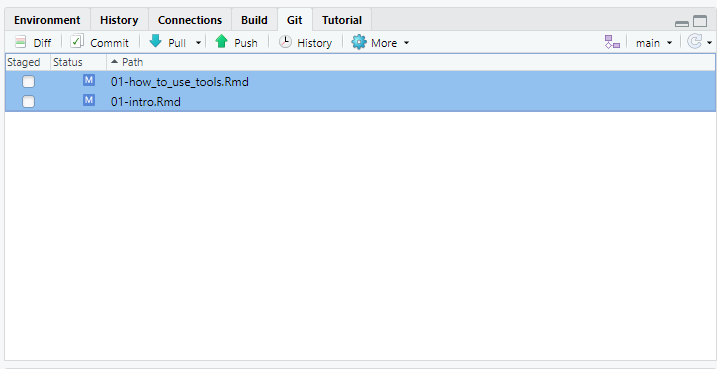
\includegraphics{01-how_to_use_tools_insertimage_1.png}

\hypertarget{tham-khux1ea3o}{%
\section{Tham khảo}\label{tham-khux1ea3o}}

\url{https://rstats.wtf/}

\hypertarget{anova-rcbd}{%
\chapter{ANOVA RCBD}\label{anova-rcbd}}

Dataset \citep{somasegaran1985}

\texttt{gs4\_deauth()} giúp cho không cần xác thực API từ googlesheet.

\href{https://docs.google.com/spreadsheets/d/1VhF7aghi8ORJHoBd8XcZvJmUeVBUliQZurGIPMkekK0/edit?usp=sharing}{File raw}

\begin{Shaded}
\begin{Highlighting}[]
\FunctionTok{library}\NormalTok{(googlesheets4)}
\FunctionTok{gs4\_deauth}\NormalTok{()}
\NormalTok{data\_rcbd }\OtherTok{\textless{}{-}} \FunctionTok{read\_sheet}\NormalTok{(}\StringTok{\textquotesingle{}1dFmKOhpYABrPR\_e5MF27W2LSbaAGdt5dFVV3zc1H47I\textquotesingle{}}\NormalTok{)}
\end{Highlighting}
\end{Shaded}

\begin{verbatim}
## v Reading from "raw_data".
\end{verbatim}

\begin{verbatim}
## v Range 'Sheet1'.
\end{verbatim}

\begin{Shaded}
\begin{Highlighting}[]
\FunctionTok{print}\NormalTok{(data\_rcbd, }\AttributeTok{n =} \ConstantTok{Inf}\NormalTok{)}
\end{Highlighting}
\end{Shaded}

\begin{verbatim}
## # A tibble: 48 x 3
##    block  treatment yield
##    <chr>  <chr>     <dbl>
##  1 block1 TAL102     9.66
##  2 block1 TAL379     9.36
##  3 block1 TAL206     8.41
##  4 block1 TAL435     8.61
##  5 block1 TAL411     9.2 
##  6 block1 ALLEN527   8.11
##  7 block1 TAL211     8.83
##  8 block1 TAL487     6.27
##  9 block1 CB1795     6.79
## 10 block1 TAL650     6.95
## 11 block1 TAL649     6.55
## 12 block1 TAL860     6   
## 13 block1 TAL183     6.11
## 14 block1 TAL378     5.39
## 15 block1 CONTROL1   1.53
## 16 block1 CONTROL2   6.41
## 17 block2 TAL102    10.6 
## 18 block2 TAL379     9   
## 19 block2 TAL206     9.44
## 20 block2 TAL435     9.23
## 21 block2 TAL411     8.19
## 22 block2 ALLEN527   8.82
## 23 block2 TAL211     6.32
## 24 block2 TAL487     8.67
## 25 block2 CB1795     8.17
## 26 block2 TAL650     5.83
## 27 block2 TAL649     4.82
## 28 block2 TAL860     4.83
## 29 block2 TAL183     3.46
## 30 block2 TAL378     4.46
## 31 block2 CONTROL1   1.3 
## 32 block2 CONTROL2   7.83
## 33 block3 TAL102    10.8 
## 34 block3 TAL379    10.5 
## 35 block3 TAL206    10.2 
## 36 block3 TAL435     8.22
## 37 block3 TAL411     8.46
## 38 block3 ALLEN527   8.62
## 39 block3 TAL211     9.14
## 40 block3 TAL487     8.35
## 41 block3 CB1795     5.7 
## 42 block3 TAL650     6.83
## 43 block3 TAL649     8.1 
## 44 block3 TAL860     6.54
## 45 block3 TAL183     5.51
## 46 block3 TAL378     5.07
## 47 block3 CONTROL1   1.8 
## 48 block3 CONTROL2   5.83
\end{verbatim}

ANOVA

\begin{Shaded}
\begin{Highlighting}[]
\FunctionTok{library}\NormalTok{(agricolae)}
\NormalTok{outAOV }\OtherTok{\textless{}{-}} \FunctionTok{aov}\NormalTok{(yield }\SpecialCharTok{\textasciitilde{}}\NormalTok{ block }\SpecialCharTok{+}\NormalTok{ treatment, }\AttributeTok{data =}\NormalTok{ data\_rcbd)}
\NormalTok{outAOV}
\end{Highlighting}
\end{Shaded}

\begin{verbatim}
## Call:
##    aov(formula = yield ~ block + treatment, data = data_rcbd)
## 
## Terms:
##                     block treatment Residuals
## Sum of Squares    2.42538 217.47868  27.94669
## Deg. of Freedom         2        15        30
## 
## Residual standard error: 0.9651716
## Estimated effects may be unbalanced
\end{verbatim}

Check assumptions

\begin{Shaded}
\begin{Highlighting}[]
\FunctionTok{plot}\NormalTok{(}\FunctionTok{fitted}\NormalTok{(outAOV), }\FunctionTok{residuals}\NormalTok{(outAOV))}
\end{Highlighting}
\end{Shaded}

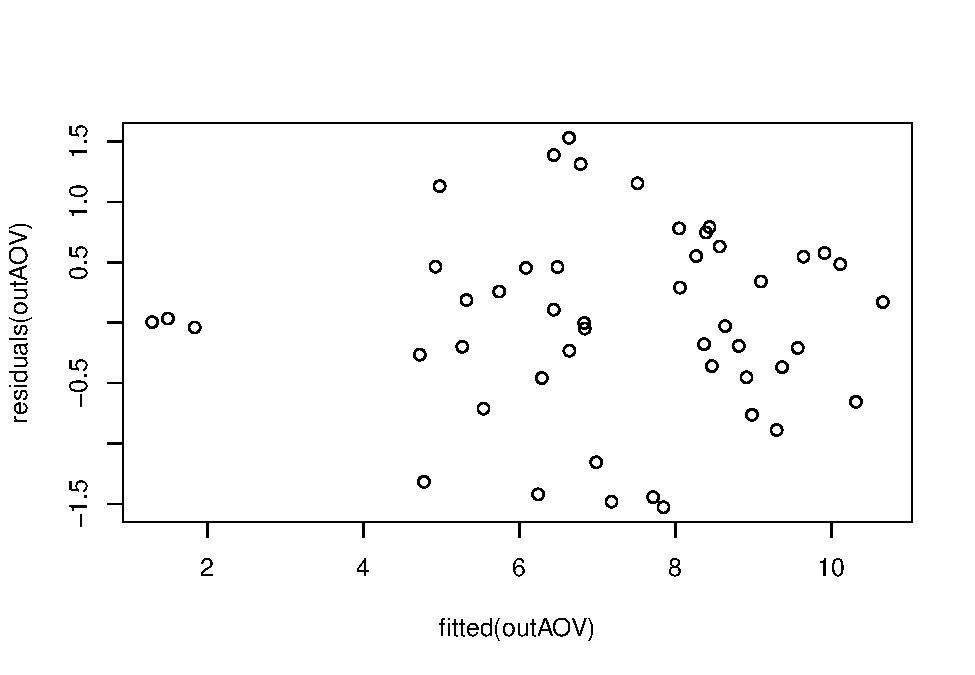
\includegraphics{_main_files/figure-latex/unnamed-chunk-5-1.pdf}

\begin{Shaded}
\begin{Highlighting}[]
\FunctionTok{hist}\NormalTok{(}\FunctionTok{residuals}\NormalTok{(outAOV))}
\FunctionTok{lines}\NormalTok{(}\FunctionTok{density}\NormalTok{(}\FunctionTok{residuals}\NormalTok{(outAOV)))}
\end{Highlighting}
\end{Shaded}

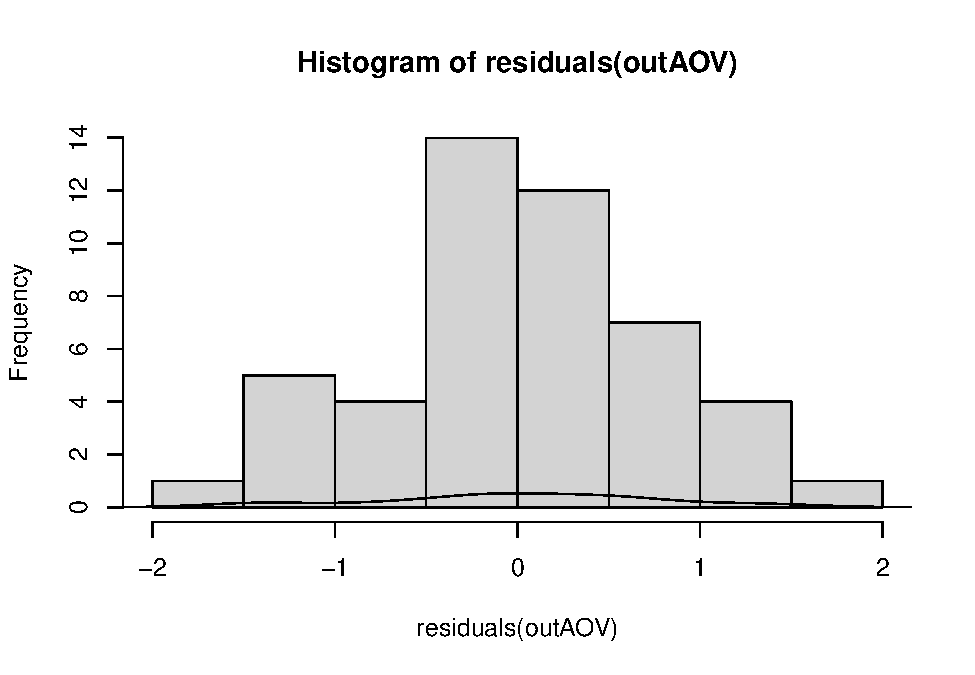
\includegraphics{_main_files/figure-latex/unnamed-chunk-5-2.pdf}

\begin{Shaded}
\begin{Highlighting}[]
\FunctionTok{hist}\NormalTok{(}\FunctionTok{residuals}\NormalTok{(outAOV), }\AttributeTok{prob =} \ConstantTok{TRUE}\NormalTok{)}
\FunctionTok{lines}\NormalTok{(}\FunctionTok{density}\NormalTok{(}\FunctionTok{residuals}\NormalTok{(outAOV)))}
\end{Highlighting}
\end{Shaded}

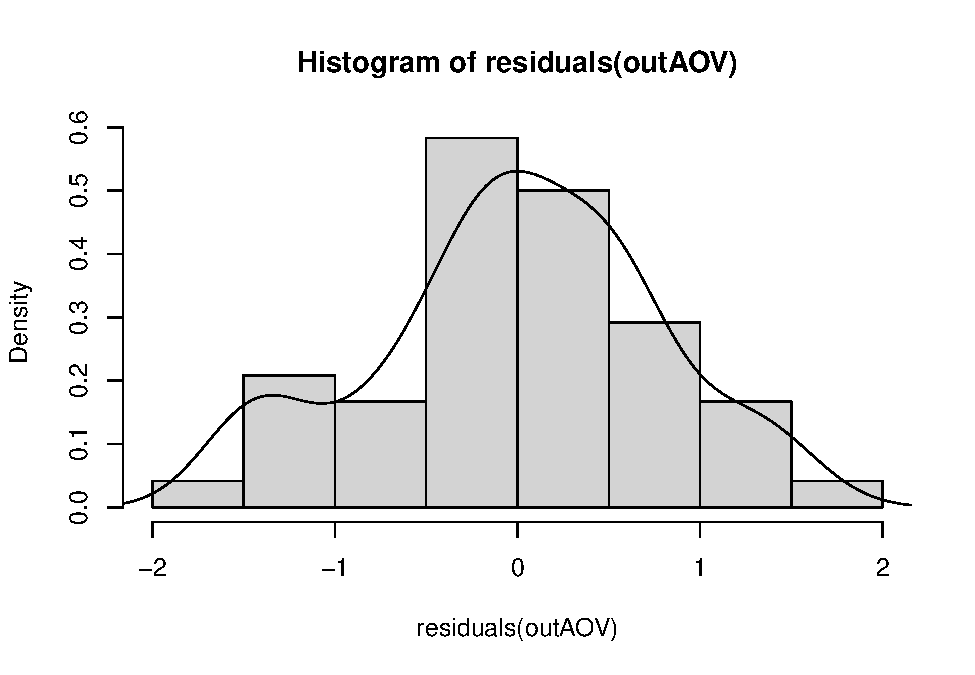
\includegraphics{_main_files/figure-latex/unnamed-chunk-5-3.pdf}

\begin{Shaded}
\begin{Highlighting}[]
\FunctionTok{library}\NormalTok{(ggpubr)}
\end{Highlighting}
\end{Shaded}

\begin{verbatim}
## Loading required package: ggplot2
\end{verbatim}

\begin{Shaded}
\begin{Highlighting}[]
\FunctionTok{ggqqplot}\NormalTok{(}\FunctionTok{residuals}\NormalTok{(outAOV))}
\end{Highlighting}
\end{Shaded}

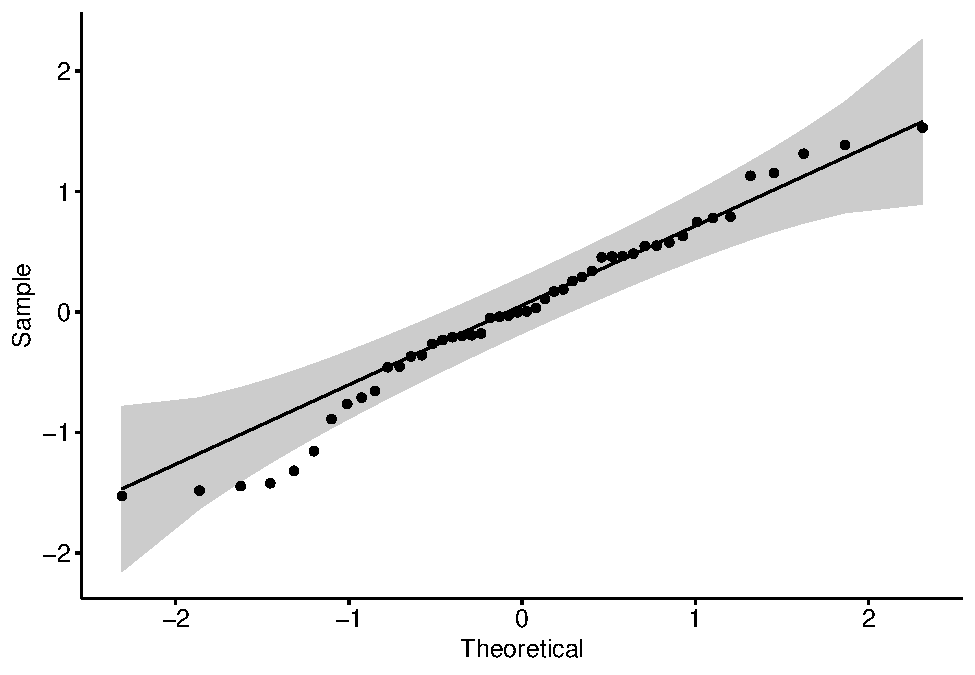
\includegraphics{_main_files/figure-latex/unnamed-chunk-5-4.pdf}

ANOVA table

\begin{Shaded}
\begin{Highlighting}[]
\FunctionTok{anova}\NormalTok{(outAOV)}
\end{Highlighting}
\end{Shaded}

\begin{verbatim}
## Analysis of Variance Table
## 
## Response: yield
##           Df  Sum Sq Mean Sq F value    Pr(>F)    
## block      2   2.425  1.2127  1.3018     0.287    
## treatment 15 217.479 14.4986 15.5638 3.284e-10 ***
## Residuals 30  27.947  0.9316                      
## ---
## Signif. codes:  0 '***' 0.001 '**' 0.01 '*' 0.05 '.' 0.1 ' ' 1
\end{verbatim}

t-test LSD

\begin{Shaded}
\begin{Highlighting}[]
\NormalTok{outFactorial }\OtherTok{\textless{}{-}}\FunctionTok{LSD.test}\NormalTok{ (outAOV, }\FunctionTok{c}\NormalTok{(}\StringTok{"treatment"}\NormalTok{), }\AttributeTok{main =} \StringTok{"yield \textasciitilde{} block + treatment"}\NormalTok{,}\AttributeTok{console=}\ConstantTok{TRUE}\NormalTok{)}
\end{Highlighting}
\end{Shaded}

\begin{verbatim}
## 
## Study: yield ~ block + treatment
## 
## LSD t Test for yield 
## 
## Mean Square Error:  0.9315563 
## 
## treatment,  means and individual ( 95 %) CI
## 
##              yield       std r       LCL       UCL  Min   Max
## ALLEN527  8.516667 0.3661056 3 7.3786265  9.654707 8.11  8.82
## CB1795    6.886667 1.2378341 3 5.7486265  8.024707 5.70  8.17
## CONTROL1  1.543333 0.2502665 3 0.4052932  2.681374 1.30  1.80
## CONTROL2  6.690000 1.0289801 3 5.5519598  7.828040 5.83  7.83
## TAL102   10.363333 0.6198656 3 9.2252932 11.501374 9.66 10.83
## TAL183    5.026667 1.3895443 3 3.8886265  6.164707 3.46  6.11
## TAL206    9.346667 0.8936629 3 8.2086265 10.484707 8.41 10.19
## TAL211    8.096667 1.5464260 3 6.9586265  9.234707 6.32  9.14
## TAL378    4.973333 0.4724757 3 3.8352932  6.111374 4.46  5.39
## TAL379    9.616667 0.7774531 3 8.4786265 10.754707 9.00 10.49
## TAL411    8.616667 0.5229085 3 7.4786265  9.754707 8.19  9.20
## TAL435    8.686667 0.5093460 3 7.5486265  9.824707 8.22  9.23
## TAL487    7.763333 1.3031245 3 6.6252932  8.901374 6.27  8.67
## TAL649    6.490000 1.6408230 3 5.3519598  7.628040 4.82  8.10
## TAL650    6.536667 0.6149255 3 5.3986265  7.674707 5.83  6.95
## TAL860    5.790000 0.8741281 3 4.6519598  6.928040 4.83  6.54
## 
## Alpha: 0.05 ; DF Error: 30
## Critical Value of t: 2.042272 
## 
## least Significant Difference: 1.609432 
## 
## Treatments with the same letter are not significantly different.
## 
##              yield groups
## TAL102   10.363333      a
## TAL379    9.616667     ab
## TAL206    9.346667    abc
## TAL435    8.686667     bc
## TAL411    8.616667     bc
## ALLEN527  8.516667     bc
## TAL211    8.096667    bcd
## TAL487    7.763333     cd
## CB1795    6.886667     de
## CONTROL2  6.690000     de
## TAL650    6.536667    def
## TAL649    6.490000    def
## TAL860    5.790000     ef
## TAL183    5.026667      f
## TAL378    4.973333      f
## CONTROL1  1.543333      g
\end{verbatim}

\hypertarget{guide}{%
\chapter{Guide}\label{guide}}

\hypertarget{inline-formatting}{%
\section{Inline formatting}\label{inline-formatting}}

\emph{work} or \emph{work}

\textbf{yes} or \textbf{yes}

H\textsubscript{2}O

Ca\textsuperscript{2+}

\texttt{code}

\textsc{Small Caps}

\href{https://www.rstudio.com}{RStudio}

Footnote\footnote{footnote}

If you do not want a certain heading to be numbered, you can add \texttt{\{-\}} after the heading, e.g \texttt{\#\ Preface\ \{-\}}

Blockquotes are written after \texttt{\textgreater{}}, e.g.,

\begin{quote}
``Love the life you live,

Live the life you love.''
--- Bob Marley
\end{quote}

\begin{verbatim}
Code blocks
\end{verbatim}

\hypertarget{listings}{%
\section{Listings}\label{listings}}

Unordered list items start with \texttt{*}, \texttt{-}, or \texttt{+}, and you can nest one list within another list by indenting the sub-list by four spaces, e.g.,

\begin{itemize}
\tightlist
\item
  one item
\item
  one item
\item
  one item

  \begin{itemize}
  \tightlist
  \item
    one item
  \item
    one item
  \end{itemize}
\end{itemize}

Ordered list items start with numbers (the rule for nested lists is the same as above), e.g.,

\begin{enumerate}
\def\labelenumi{\arabic{enumi}.}
\tightlist
\item
  the first item
\item
  the second item
\item
  the third item
\end{enumerate}

\hypertarget{media}{%
\section{Media}\label{media}}

\href{https://t.me/inspiring_melody/321}{Mình cưới thôi em}

\hypertarget{images}{%
\section{Images}\label{images}}

\begin{itemize}
\item
  Chèn theo syntax trong markdown
  
\includegraphics{images/heart.png}
\item
  Chèn từ link sử dụng thẻ \texttt{HTML}
  \texttt{\textless{}img\ src="link.png"\ alt="caption"\ style="height:\ 100px;\ width:100px;"/\textgreater{}}
\end{itemize}

Xem thêm \url{https://www.markdownguide.org/hacks/\#image-size}

\hypertarget{math-expressions}{%
\section{Math expressions}\label{math-expressions}}

Ma trận dãy số

\[\begin{array}{ccc}
x_{11} & x_{12} & x_{13}\\
x_{21} & x_{22} & x_{23}
\end{array}\]

Ma trận

\[X = \begin{bmatrix}1 & x_{1}\\
1 & x_{2}\\
1 & x_{3}
\end{bmatrix}\]

\[\Theta = \begin{pmatrix}\alpha & \beta\\
\gamma & \delta
\end{pmatrix}\]

\[\begin{vmatrix}a & b\\
c & d
\end{vmatrix}=ad-bc\]

\hypertarget{number-and-reference-equations}{%
\section{Number and reference equations}\label{number-and-reference-equations}}

\begin{equation} 
  f\left(k\right) = \binom{n}{k} p^k\left(1-p\right)^{n-k}
  \label{eq:binom}
\end{equation}

You may refer to it using \texttt{\textbackslash{}@ref(eq:binom)}, e.g., see Equation \eqref{eq:binom}.

Công thức mô tả a normal frequency curve

\begin{equation} 
  f = \frac{N}{{(\sigma \sqrt {2\pi } )}}{e^{ - {{(y - \mu )}^2}/2{\sigma ^2}}}
  \label{eq:normal}
\end{equation}

You may refer to it using \texttt{\textbackslash{}@ref(eq:normal)}, e.g., see Equation \eqref{eq:normal}.

Nếu không đánh số công thức thì dùng \texttt{equation*}

\begin{equation*} 
\frac{d}{dx}\left( \int_{a}^{x} f(u)\,du\right)=f(x)
\end{equation*}

Nếu ghi theo kiểu \texttt{align} thì áp dụng

\begin{align} 
g(X_{n}) &= g(\theta)+g'({\tilde{\theta}})(X_{n}-\theta) \notag \\

\sqrt{n}[g(X_{n})-g(\theta)] &= g'\left({\tilde{\theta}}\right)
  \sqrt{n}[X_{n}-\theta ] 

\label{eq:align}
\end{align}

Sử dụng \texttt{\textbackslash{}notag} để giúp không đánh số công thức ở hàng đầu tiên của \eqref{eq:align}

Nếu sử dụng \texttt{split} thì áp dụng

\begin{equation} 
\begin{split}
\mathrm{Var}(\hat{\beta}) & =\mathrm{Var}((X'X)^{-1}X'y)\\
 & =(X'X)^{-1}X'\mathrm{Var}(y)((X'X)^{-1}X')'\\
 & =(X'X)^{-1}X'\mathrm{Var}(y)X(X'X)^{-1}\\
 & =(X'X)^{-1}X'\sigma^{2}IX(X'X)^{-1}\\
 & =(X'X)^{-1}\sigma^{2}
\end{split}
\label{eq:var-beta}
\end{equation}

\hypertarget{theorems-and-proofs}{%
\section{Theorems and proofs}\label{theorems-and-proofs}}

\begin{theorem}[Pythagorean theorem]
For a right triangle, if \(c\) denotes the length of the hypotenuse
and \(a\) and \(b\) denote the lengths of the other two sides, we have
\[a^2 + b^2 = c^2\]
\end{theorem}

\hypertarget{text-references}{%
\section{Text references}\label{text-references}}

You can assign some text to a label and reference the text using the label elsewhere in your document. This can be particularly useful for long figure/table captions.

\hypertarget{r-code}{%
\section{R code}\label{r-code}}

There are two types of R code in R Markdown/knitr documents: R code chunks, and inline R code. The syntax for the latter is \texttt{\textasciigrave{}r\ R\_CODE\textasciigrave{}}, and it can be embedded inline with other document elements.

\hypertarget{figures}{%
\section{Figures}\label{figures}}

If we assign a figure caption to a code chunk via the chunk option \texttt{fig.cap}, R plots will be put into figure environments, which will be automatically labeled and numbered, and can also be cross-referenced. The label of a figure environment is generated from the label of the code chunk.

Cross reference cho Figure \ref{fig:pressure-plot}

\begin{Shaded}
\begin{Highlighting}[]
\FunctionTok{par}\NormalTok{(}\AttributeTok{mar =} \FunctionTok{c}\NormalTok{(}\DecValTok{4}\NormalTok{, }\DecValTok{4}\NormalTok{, .}\DecValTok{1}\NormalTok{, .}\DecValTok{1}\NormalTok{))}
\FunctionTok{plot}\NormalTok{(pressure, }\AttributeTok{pch =} \DecValTok{19}\NormalTok{, }\AttributeTok{type =} \StringTok{\textquotesingle{}b\textquotesingle{}}\NormalTok{)}
\end{Highlighting}
\end{Shaded}

\begin{figure}

{\centering 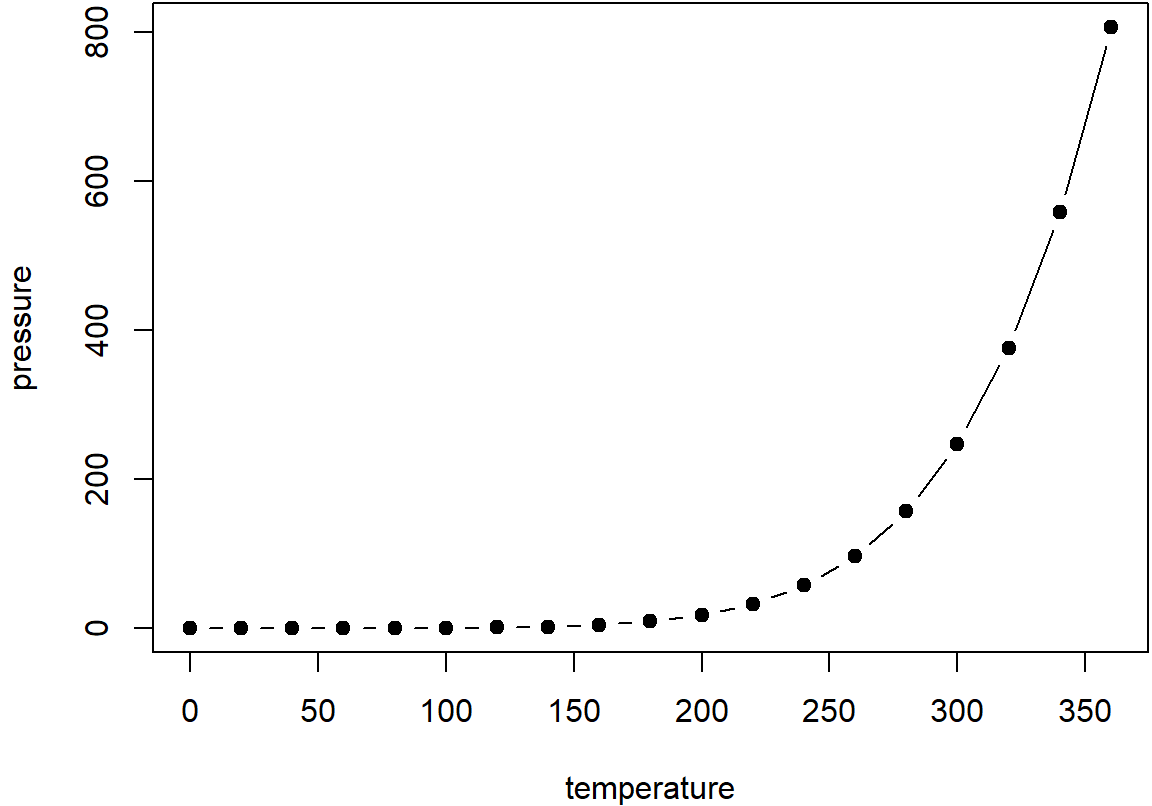
\includegraphics[width=0.9\linewidth]{_main_files/figure-latex/pressure-plot-1} 

}

\caption{A figure example with the specified aspect ratio, width, and alignment.}\label{fig:pressure-plot}
\end{figure}

Chèn hai đồ thị \ref{fig:multi-plots}

\begin{Shaded}
\begin{Highlighting}[]
\FunctionTok{par}\NormalTok{(}\AttributeTok{mar =} \FunctionTok{c}\NormalTok{(}\DecValTok{4}\NormalTok{, }\DecValTok{4}\NormalTok{, .}\DecValTok{1}\NormalTok{, .}\DecValTok{1}\NormalTok{))}
\FunctionTok{plot}\NormalTok{(pressure, }\AttributeTok{pch =} \DecValTok{19}\NormalTok{, }\AttributeTok{type =} \StringTok{\textquotesingle{}b\textquotesingle{}}\NormalTok{)}
\FunctionTok{plot}\NormalTok{(cars, }\AttributeTok{pch =} \DecValTok{19}\NormalTok{)}
\end{Highlighting}
\end{Shaded}

\begin{figure}
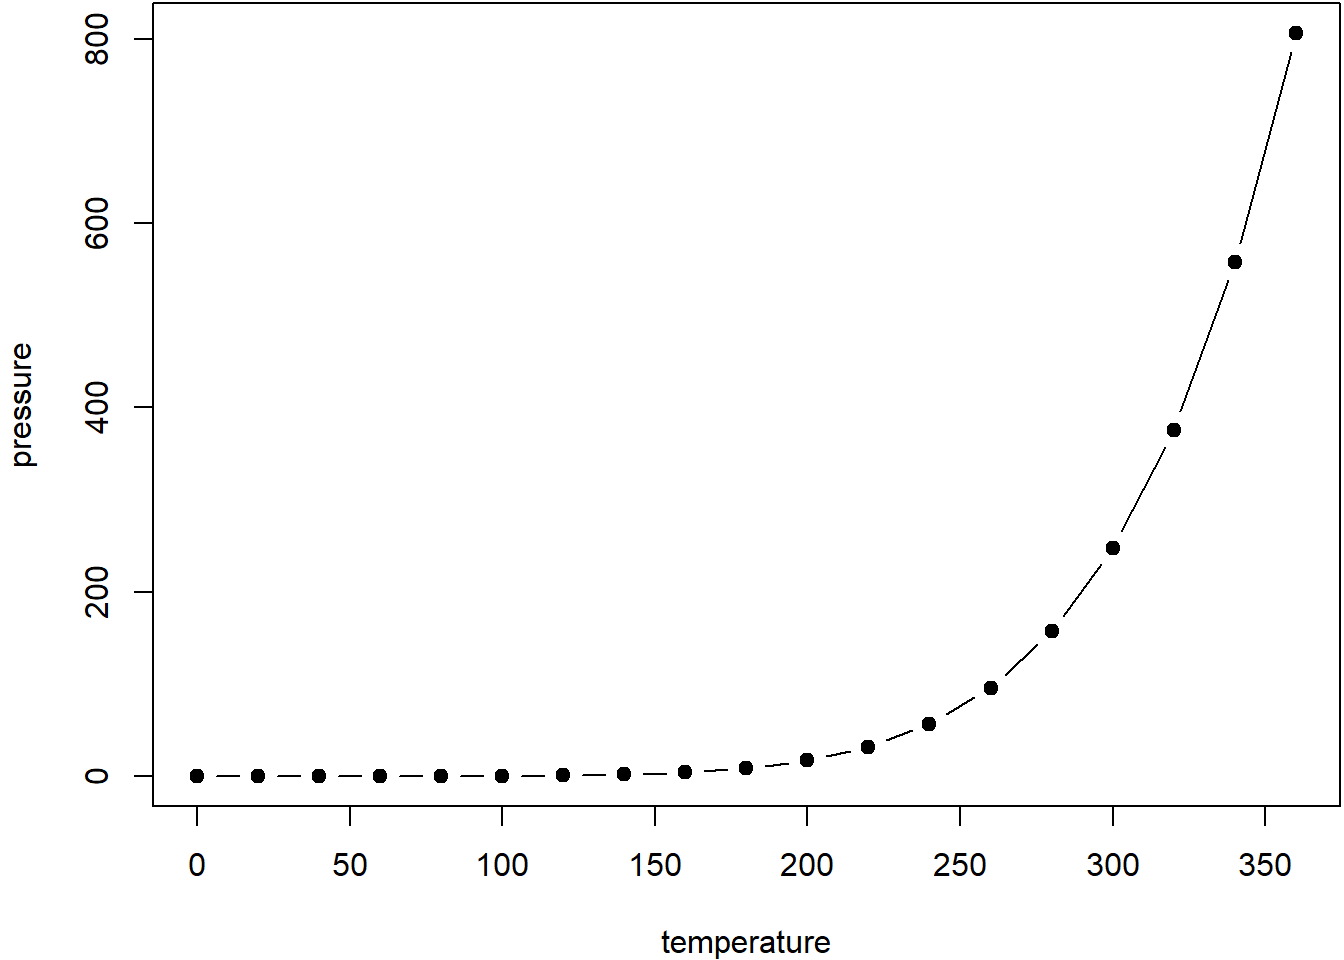
\includegraphics[width=0.5\linewidth]{_main_files/figure-latex/multi-plots-1} 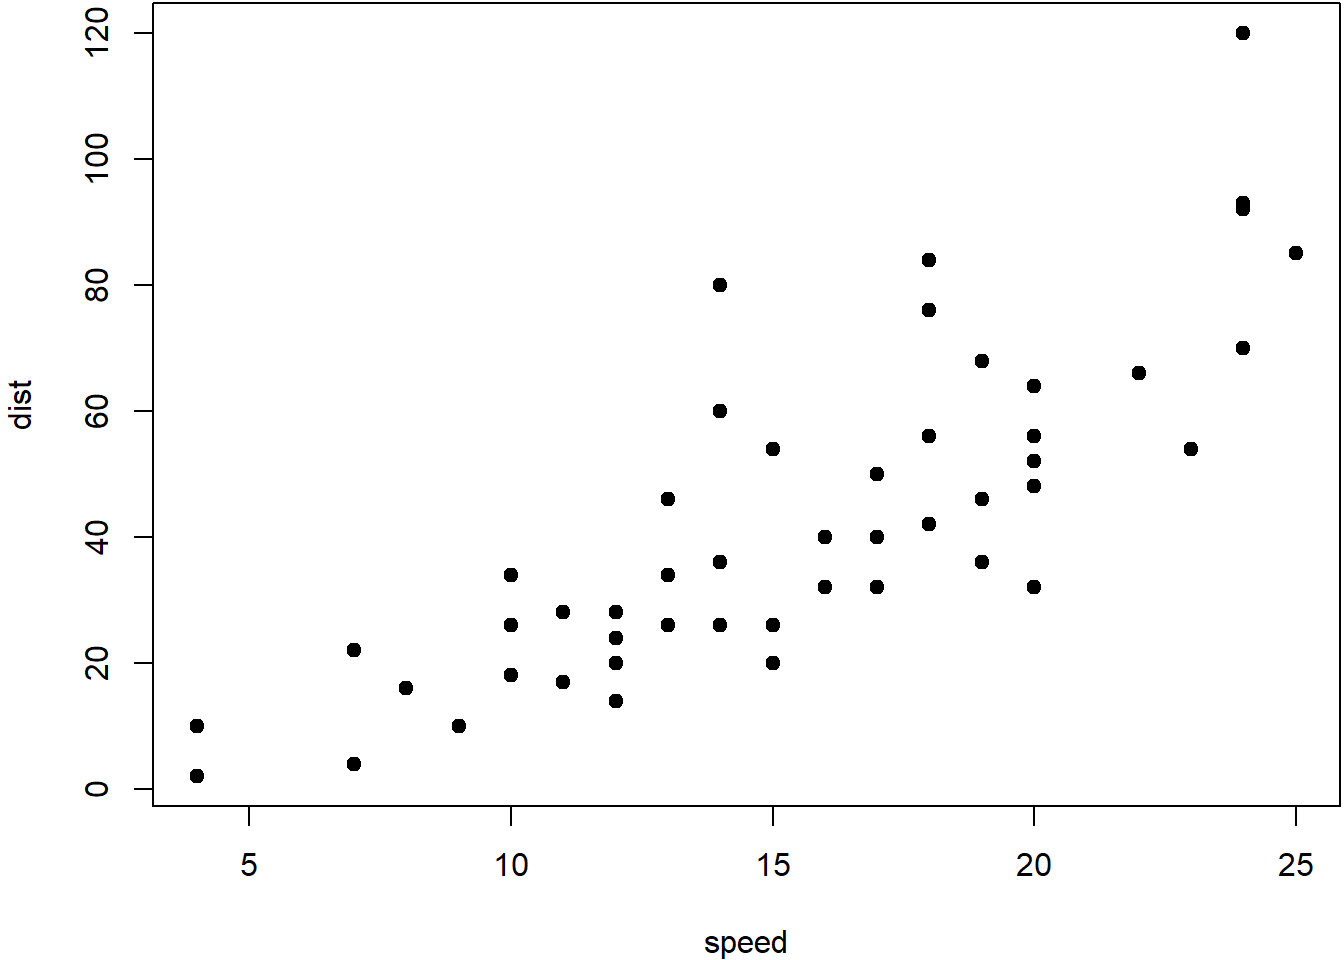
\includegraphics[width=0.5\linewidth]{_main_files/figure-latex/multi-plots-2} \caption{Two plots placed side by side.}\label{fig:multi-plots}
\end{figure}

Chèn hình ảnh

\begin{Shaded}
\begin{Highlighting}[]
\NormalTok{knitr}\SpecialCharTok{::}\FunctionTok{include\_graphics}\NormalTok{(}\StringTok{\textquotesingle{}images/michael.jpg\textquotesingle{}}\NormalTok{)}
\end{Highlighting}
\end{Shaded}

\begin{figure}

\includegraphics[width=0.328\linewidth]{images/michael} \caption{Never let anyone know your mind.}\label{fig:michael}
\end{figure}

Chèn lặp lại hình ảnh

\begin{Shaded}
\begin{Highlighting}[]
\NormalTok{knitr}\SpecialCharTok{::}\FunctionTok{include\_graphics}\NormalTok{(}\FunctionTok{rep}\NormalTok{(}\StringTok{\textquotesingle{}images/turtle.jpg\textquotesingle{}}\NormalTok{, }\DecValTok{3}\NormalTok{))}
\end{Highlighting}
\end{Shaded}

\begin{figure}
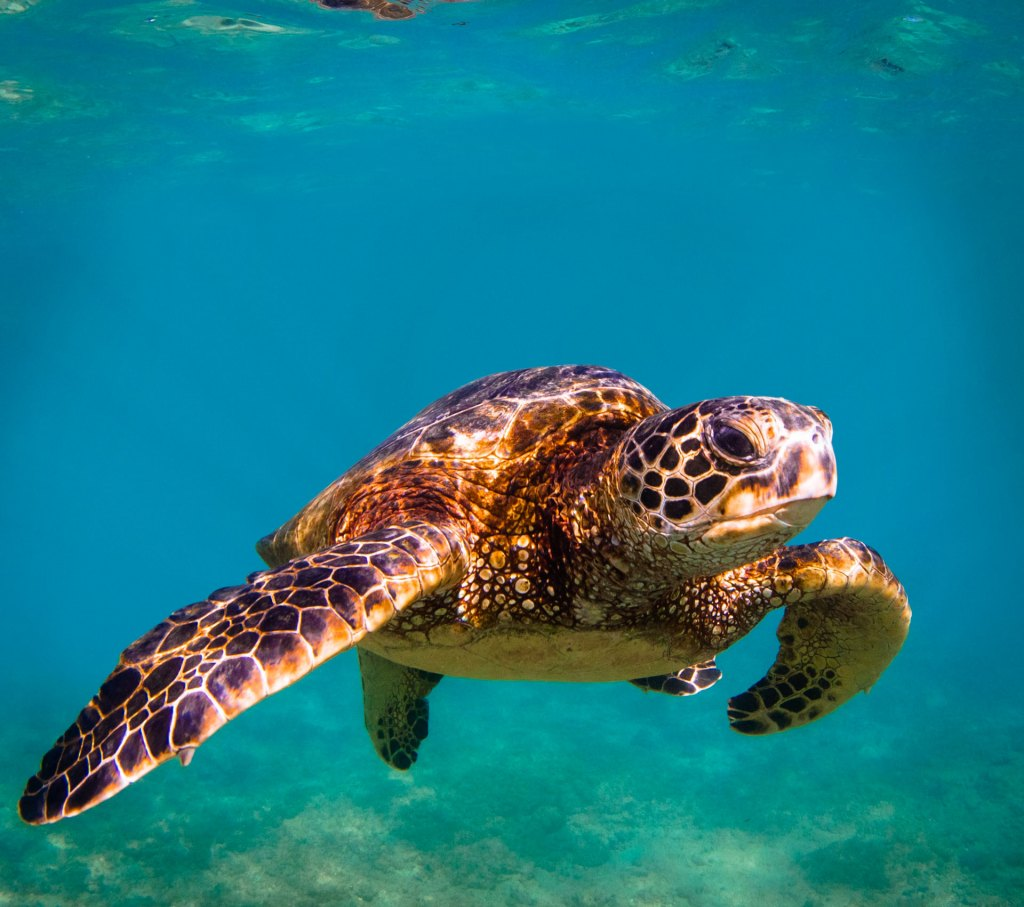
\includegraphics[width=0.328\linewidth]{images/turtle} 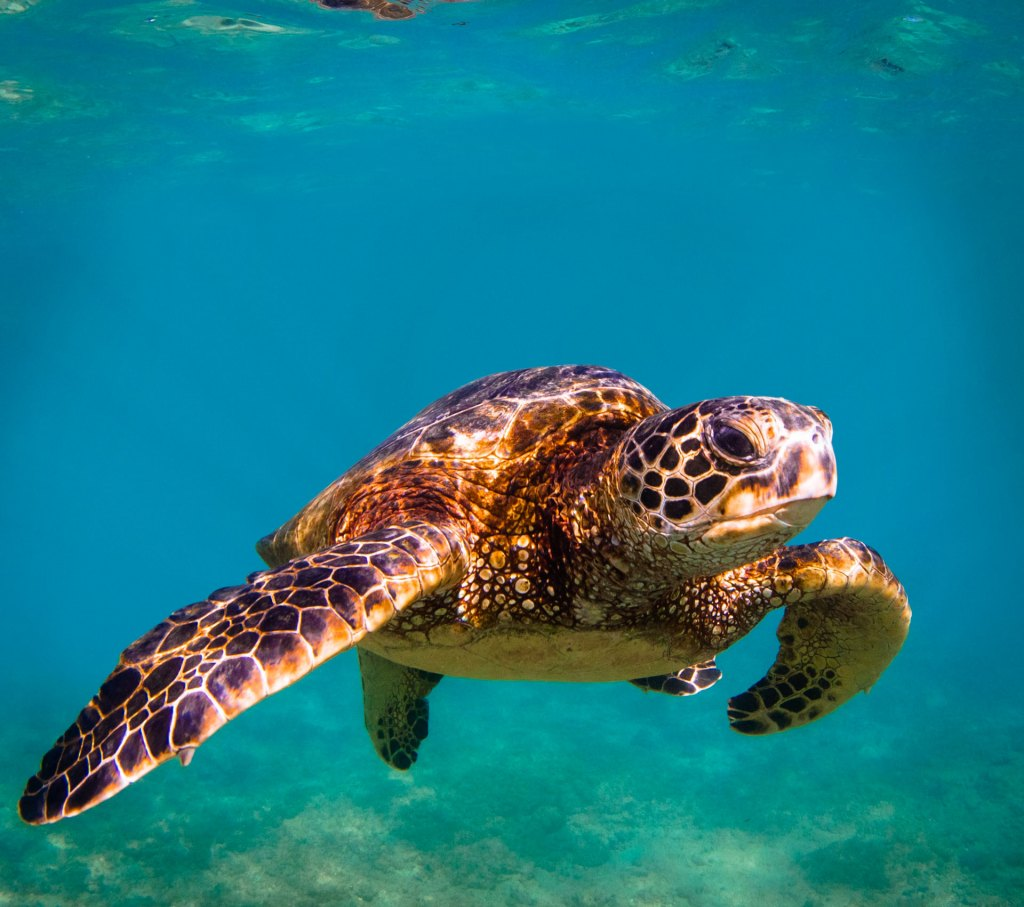
\includegraphics[width=0.328\linewidth]{images/turtle} 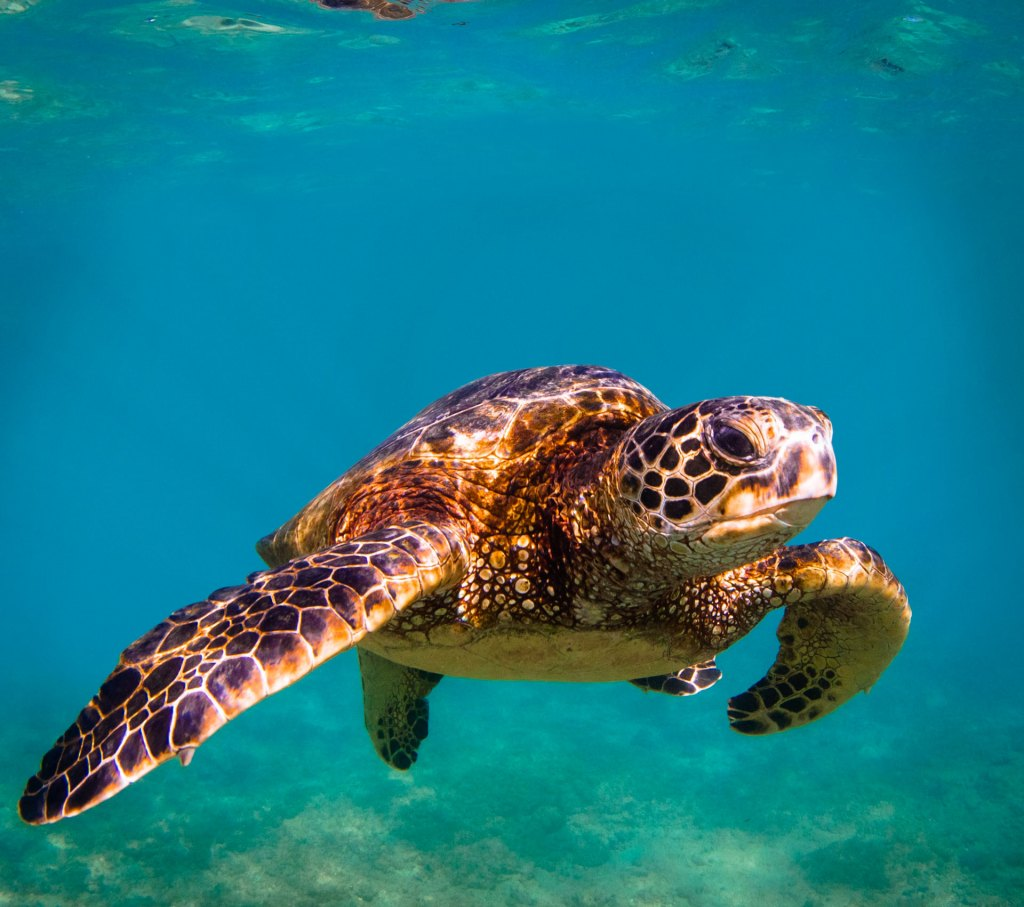
\includegraphics[width=0.328\linewidth]{images/turtle} \caption{Finding good land.}\label{fig:turtle}
\end{figure}

\hypertarget{tables}{%
\section{Tables}\label{tables}}

Like figures, tables with captions will also be numbered and can be referenced.

Table \ref{tab:table-single} is a simple example.

\begin{Shaded}
\begin{Highlighting}[]
\NormalTok{knitr}\SpecialCharTok{::}\FunctionTok{kable}\NormalTok{(}
  \FunctionTok{head}\NormalTok{(mtcars[, }\DecValTok{1}\SpecialCharTok{:}\DecValTok{8}\NormalTok{], }\DecValTok{10}\NormalTok{), }\AttributeTok{booktabs =} \ConstantTok{TRUE}\NormalTok{,}
  \AttributeTok{caption =} \StringTok{\textquotesingle{}A table of the first 10 rows of the mtcars data.\textquotesingle{}}
\NormalTok{)}
\end{Highlighting}
\end{Shaded}

\begin{table}

\caption{\label{tab:table-single}A table of the first 10 rows of the mtcars data.}
\centering
\begin{tabular}[t]{lrrrrrrrr}
\toprule
  & mpg & cyl & disp & hp & drat & wt & qsec & vs\\
\midrule
Mazda RX4 & 21.0 & 6 & 160.0 & 110 & 3.90 & 2.620 & 16.46 & 0\\
Mazda RX4 Wag & 21.0 & 6 & 160.0 & 110 & 3.90 & 2.875 & 17.02 & 0\\
Datsun 710 & 22.8 & 4 & 108.0 & 93 & 3.85 & 2.320 & 18.61 & 1\\
Hornet 4 Drive & 21.4 & 6 & 258.0 & 110 & 3.08 & 3.215 & 19.44 & 1\\
Hornet Sportabout & 18.7 & 8 & 360.0 & 175 & 3.15 & 3.440 & 17.02 & 0\\
\addlinespace
Valiant & 18.1 & 6 & 225.0 & 105 & 2.76 & 3.460 & 20.22 & 1\\
Duster 360 & 14.3 & 8 & 360.0 & 245 & 3.21 & 3.570 & 15.84 & 0\\
Merc 240D & 24.4 & 4 & 146.7 & 62 & 3.69 & 3.190 & 20.00 & 1\\
Merc 230 & 22.8 & 4 & 140.8 & 95 & 3.92 & 3.150 & 22.90 & 1\\
Merc 280 & 19.2 & 6 & 167.6 & 123 & 3.92 & 3.440 & 18.30 & 1\\
\bottomrule
\end{tabular}
\end{table}

If you want to put multiple tables in a single table environment, wrap the data objects (usually data frames in R) into a list. See Table \ref{tab:table-multi} for an example. Please note that this feature is only available in HTML and PDF output.

\begin{Shaded}
\begin{Highlighting}[]
\NormalTok{knitr}\SpecialCharTok{::}\FunctionTok{kable}\NormalTok{(}
  \FunctionTok{list}\NormalTok{(}
    \FunctionTok{head}\NormalTok{(iris[, }\DecValTok{1}\SpecialCharTok{:}\DecValTok{2}\NormalTok{], }\DecValTok{3}\NormalTok{),}
    \FunctionTok{head}\NormalTok{(mtcars[, }\DecValTok{1}\SpecialCharTok{:}\DecValTok{3}\NormalTok{], }\DecValTok{5}\NormalTok{)}
\NormalTok{  ),}
  \AttributeTok{caption =} \StringTok{\textquotesingle{}A Tale of Two Tables.\textquotesingle{}}\NormalTok{, }\AttributeTok{booktabs =} \ConstantTok{TRUE}
\NormalTok{)}
\end{Highlighting}
\end{Shaded}

\begin{table}
\caption{\label{tab:table-multi}A Tale of Two Tables.}

\centering
\begin{tabular}[t]{rr}
\toprule
Sepal.Length & Sepal.Width\\
\midrule
5.1 & 3.5\\
4.9 & 3.0\\
4.7 & 3.2\\
\bottomrule
\end{tabular}
\centering
\begin{tabular}[t]{lrrr}
\toprule
  & mpg & cyl & disp\\
\midrule
Mazda RX4 & 21.0 & 6 & 160\\
Mazda RX4 Wag & 21.0 & 6 & 160\\
Datsun 710 & 22.8 & 4 & 108\\
Hornet 4 Drive & 21.4 & 6 & 258\\
Hornet Sportabout & 18.7 & 8 & 360\\
\bottomrule
\end{tabular}
\end{table}

Longtable. Nếu dùng trong HTML thì áp dụng đoạn code. Còn nếu dùng trong PDF thì add \texttt{\textbackslash{}usepackage\{longtable\}} vào phần LaTeX preamble.

\begin{Shaded}
\begin{Highlighting}[]
\NormalTok{knitr}\SpecialCharTok{::}\FunctionTok{kable}\NormalTok{(}
\NormalTok{  iris[}\DecValTok{1}\SpecialCharTok{:}\DecValTok{55}\NormalTok{, ], }\AttributeTok{longtable =} \ConstantTok{TRUE}\NormalTok{, }\AttributeTok{booktabs =} \ConstantTok{TRUE}\NormalTok{,}
  \AttributeTok{caption =} \StringTok{\textquotesingle{}A table generated by the longtable package.\textquotesingle{}}
\NormalTok{)}
\end{Highlighting}
\end{Shaded}

\begin{longtable}[t]{rrrrl}
\caption{\label{tab:longtable}A table generated by the longtable package.}\\
\toprule
Sepal.Length & Sepal.Width & Petal.Length & Petal.Width & Species\\
\midrule
5.1 & 3.5 & 1.4 & 0.2 & setosa\\
4.9 & 3.0 & 1.4 & 0.2 & setosa\\
4.7 & 3.2 & 1.3 & 0.2 & setosa\\
4.6 & 3.1 & 1.5 & 0.2 & setosa\\
5.0 & 3.6 & 1.4 & 0.2 & setosa\\
\addlinespace
5.4 & 3.9 & 1.7 & 0.4 & setosa\\
4.6 & 3.4 & 1.4 & 0.3 & setosa\\
5.0 & 3.4 & 1.5 & 0.2 & setosa\\
4.4 & 2.9 & 1.4 & 0.2 & setosa\\
4.9 & 3.1 & 1.5 & 0.1 & setosa\\
\addlinespace
5.4 & 3.7 & 1.5 & 0.2 & setosa\\
4.8 & 3.4 & 1.6 & 0.2 & setosa\\
4.8 & 3.0 & 1.4 & 0.1 & setosa\\
4.3 & 3.0 & 1.1 & 0.1 & setosa\\
5.8 & 4.0 & 1.2 & 0.2 & setosa\\
\addlinespace
5.7 & 4.4 & 1.5 & 0.4 & setosa\\
5.4 & 3.9 & 1.3 & 0.4 & setosa\\
5.1 & 3.5 & 1.4 & 0.3 & setosa\\
5.7 & 3.8 & 1.7 & 0.3 & setosa\\
5.1 & 3.8 & 1.5 & 0.3 & setosa\\
\addlinespace
5.4 & 3.4 & 1.7 & 0.2 & setosa\\
5.1 & 3.7 & 1.5 & 0.4 & setosa\\
4.6 & 3.6 & 1.0 & 0.2 & setosa\\
5.1 & 3.3 & 1.7 & 0.5 & setosa\\
4.8 & 3.4 & 1.9 & 0.2 & setosa\\
\addlinespace
5.0 & 3.0 & 1.6 & 0.2 & setosa\\
5.0 & 3.4 & 1.6 & 0.4 & setosa\\
5.2 & 3.5 & 1.5 & 0.2 & setosa\\
5.2 & 3.4 & 1.4 & 0.2 & setosa\\
4.7 & 3.2 & 1.6 & 0.2 & setosa\\
\addlinespace
4.8 & 3.1 & 1.6 & 0.2 & setosa\\
5.4 & 3.4 & 1.5 & 0.4 & setosa\\
5.2 & 4.1 & 1.5 & 0.1 & setosa\\
5.5 & 4.2 & 1.4 & 0.2 & setosa\\
4.9 & 3.1 & 1.5 & 0.2 & setosa\\
\addlinespace
5.0 & 3.2 & 1.2 & 0.2 & setosa\\
5.5 & 3.5 & 1.3 & 0.2 & setosa\\
4.9 & 3.6 & 1.4 & 0.1 & setosa\\
4.4 & 3.0 & 1.3 & 0.2 & setosa\\
5.1 & 3.4 & 1.5 & 0.2 & setosa\\
\addlinespace
5.0 & 3.5 & 1.3 & 0.3 & setosa\\
4.5 & 2.3 & 1.3 & 0.3 & setosa\\
4.4 & 3.2 & 1.3 & 0.2 & setosa\\
5.0 & 3.5 & 1.6 & 0.6 & setosa\\
5.1 & 3.8 & 1.9 & 0.4 & setosa\\
\addlinespace
4.8 & 3.0 & 1.4 & 0.3 & setosa\\
5.1 & 3.8 & 1.6 & 0.2 & setosa\\
4.6 & 3.2 & 1.4 & 0.2 & setosa\\
5.3 & 3.7 & 1.5 & 0.2 & setosa\\
5.0 & 3.3 & 1.4 & 0.2 & setosa\\
\addlinespace
7.0 & 3.2 & 4.7 & 1.4 & versicolor\\
6.4 & 3.2 & 4.5 & 1.5 & versicolor\\
6.9 & 3.1 & 4.9 & 1.5 & versicolor\\
5.5 & 2.3 & 4.0 & 1.3 & versicolor\\
6.5 & 2.8 & 4.6 & 1.5 & versicolor\\
\bottomrule
\end{longtable}

Tạo table thủ công. Table \ref{tab:manual}

\begin{longtable}[]{@{}rrrr@{}}
\caption{\label{tab:manual} A simple table in Markdown.}\tabularnewline
\toprule
Sepal.Length & Sepal.Width & Petal.Length & Petal.Width \\
\midrule
\endfirsthead
\toprule
Sepal.Length & Sepal.Width & Petal.Length & Petal.Width \\
\midrule
\endhead
5.1 & 3.5 & 1.4 & 0.2 \\
4.9 & 3.0 & 1.4 & 0.2 \\
4.7 & 3.2 & 1.3 & 0.2 \\
4.6 & 3.1 & 1.5 & 0.2 \\
5.0 & 3.6 & 1.4 & 0.2 \\
5.4 & 3.9 & 1.7 & 0.4 \\
\bottomrule
\end{longtable}

\hypertarget{basic-blocks}{%
\chapter{Basic blocks}\label{basic-blocks}}

\hypertarget{subsets}{%
\section{Subsets}\label{subsets}}

Nguồn \citep[p.~241]{devriesDummies2015}

\begin{Shaded}
\begin{Highlighting}[]
\FunctionTok{str}\NormalTok{(islands)}
\end{Highlighting}
\end{Shaded}

\begin{verbatim}
##  Named num [1:48] 11506 5500 16988 2968 16 ...
##  - attr(*, "names")= chr [1:48] "Africa" "Antarctica" "Asia" "Australia" ...
\end{verbatim}

\begin{Shaded}
\begin{Highlighting}[]
\NormalTok{islands}
\end{Highlighting}
\end{Shaded}

\begin{verbatim}
##           Africa       Antarctica             Asia        Australia 
##            11506             5500            16988             2968 
##     Axel Heiberg           Baffin            Banks           Borneo 
##               16              184               23              280 
##          Britain          Celebes            Celon             Cuba 
##               84               73               25               43 
##            Devon        Ellesmere           Europe        Greenland 
##               21               82             3745              840 
##           Hainan       Hispaniola         Hokkaido           Honshu 
##               13               30               30               89 
##          Iceland          Ireland             Java           Kyushu 
##               40               33               49               14 
##            Luzon       Madagascar         Melville         Mindanao 
##               42              227               16               36 
##         Moluccas      New Britain       New Guinea  New Zealand (N) 
##               29               15              306               44 
##  New Zealand (S)     Newfoundland    North America    Novaya Zemlya 
##               58               43             9390               32 
##  Prince of Wales         Sakhalin    South America      Southampton 
##               13               29             6795               16 
##      Spitsbergen          Sumatra           Taiwan         Tasmania 
##               15              183               14               26 
## Tierra del Fuego            Timor        Vancouver         Victoria 
##               19               13               12               82
\end{verbatim}

\begin{figure}
\centering
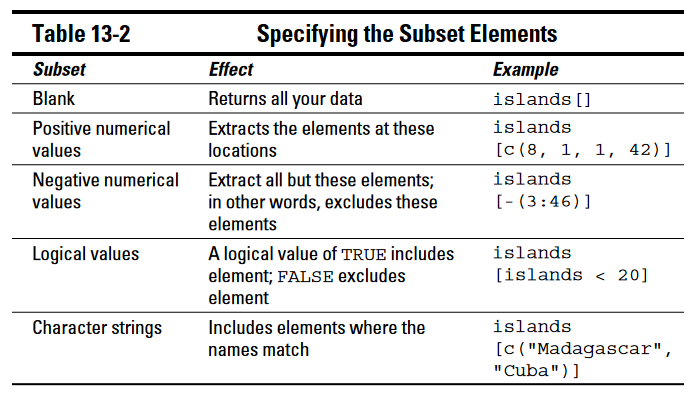
\includegraphics{images/subset1.png}
\caption{Subset elements}
\end{figure}

\hypertarget{example-1}{%
\chapter{EXAMPLE 1}\label{example-1}}

Source: Programming Assignment 3 INSTRUCTIONS: Hospital Quality {[}R Programming Coursera{]}

Idea: \href{https://tanduc307.github.io/xstk/example/1/idea_rprog_data_ProgAssignment3-data.pdf}{Yêu cầu đề bài}

Download data: \href{https://tanduc307.github.io/xstk/example/1/rprog_data_ProgAssignment3-data.zip}{Dữ liệu đề bài}

\hypertarget{download-data}{%
\section{DOWNLOAD DATA}\label{download-data}}

\begin{Shaded}
\begin{Highlighting}[]
\ControlFlowTok{if}\NormalTok{(}\SpecialCharTok{!}\FunctionTok{file.exists}\NormalTok{(}\StringTok{"./example/1/rprog\_data\_ProgAssignment3{-}data.zip"}\NormalTok{)) }\CommentTok{\# KIỂM TRA XEM CÓ FILE NÀY ĐÃ DOWNLOAD TRONG THƯ MỤC CHƯA}
  
  \CommentTok{\# NẾU CHƯA CÓ THÌ TIẾN HÀNH DOWNLOAD VÀ GIẢI NÉN}
  
\NormalTok{  \{}
  
\NormalTok{  url }\OtherTok{\textless{}{-}} \StringTok{"https://tanduc307.github.io/xstk/example/1/rprog\_data\_ProgAssignment3{-}data.zip"} \CommentTok{\# GÁN GIÁ TRỊ LINK DOWNLOAD}
  \FunctionTok{library}\NormalTok{(here) }\CommentTok{\# SỬ DỤNG PACKAGE \textquotesingle{}here\textquotesingle{} ĐỂ TẠO ĐƯỜNG DẪN CHO TIỆN}
\NormalTok{  working\_wd }\OtherTok{\textless{}{-}} \FunctionTok{getwd}\NormalTok{() }\CommentTok{\# GÁN GIÁ TRỊ THƯ MỤC LÀM VIỆC}
\NormalTok{  destfile }\OtherTok{\textless{}{-}} \FunctionTok{here}\NormalTok{(working\_wd, }\StringTok{"example"}\NormalTok{, }\StringTok{"1"}\NormalTok{, }\StringTok{"rprog\_data\_ProgAssignment3{-}data.zip"}\NormalTok{) }\CommentTok{\# GÁN GIÁ TRỊ VỊ TRÍ FILE SẼ DOWNLOAD}
  
  \FunctionTok{download.file}\NormalTok{(url, destfile) }\CommentTok{\# DOWNLOAD FILE VỀ THƯ MỤC LÀM VIỆC}
  
\NormalTok{  unzip\_folder }\OtherTok{\textless{}{-}} \FunctionTok{here}\NormalTok{(working\_wd, }\StringTok{"example"}\NormalTok{, }\StringTok{"1"}\NormalTok{) }\CommentTok{\# GÁN GIÁ TRỊ VỊ TRÍ FILE SẼ GIẢI NÉN}
  \FunctionTok{unzip}\NormalTok{(}\AttributeTok{zipfile =}\NormalTok{ destfile, }\AttributeTok{exdir =}\NormalTok{ unzip\_folder) }\CommentTok{\# GIẢI NÉN FILE}
  \FunctionTok{list.files}\NormalTok{(unzip\_folder) }\CommentTok{\# LIỆT KÊ CÁC FILE TRONG THƯ MỤC SAU GIẢI NÉN}
  
\NormalTok{  \} }\CommentTok{\# KẾT THÚC HÀM IF}
\end{Highlighting}
\end{Shaded}

\hypertarget{giux1ea3i-buxe0i-tux1eadp}{%
\section{GIẢI BÀI TẬP}\label{giux1ea3i-buxe0i-tux1eadp}}

Bạn nên dùng MS Excel để mở các bảng dữ liệu này ra để có cái nhìn về toàn bộ dữ liệu và cách trích xuất dữ liệu thủ công theo yêu cầu đề bài sẽ gồm những bước nào. Từ đây khi viết hàm vào R sẽ có thể dễ dàng đối chiếu kết quả.

\hypertarget{tuxecm-ra-bang-nuxe0o-cuxf3-tux1ef7-lux1ec7-bux1ec7nh-thux1ea5p-nhux1ea5t}{%
\subsection{TÌM RA BANG NÀO CÓ TỶ LỆ BỆNH THẤP NHẤT}\label{tuxecm-ra-bang-nuxe0o-cuxf3-tux1ef7-lux1ec7-bux1ec7nh-thux1ea5p-nhux1ea5t}}

Lưu hàm ở file best.R

\begin{Shaded}
\begin{Highlighting}[]
\NormalTok{best }\OtherTok{\textless{}{-}} \ControlFlowTok{function}\NormalTok{(state\_real, outcome\_real) }

  \CommentTok{\# ĐẶT HÀM TÊN LÀ \textquotesingle{}best\textquotesingle{}, CÓ HAI THÔNG SỐ LÀ \textquotesingle{}state\_real\textquotesingle{} là tên của bang; \textquotesingle{}outcome\_real\textquotesingle{} là tỷ lệ bệnh.  }
  
\NormalTok{  \{}
  
  \CommentTok{\# NHẬP DỮ LIỆU}
  \FunctionTok{library}\NormalTok{(here)}
\NormalTok{  working\_wd }\OtherTok{\textless{}{-}} \FunctionTok{getwd}\NormalTok{()}
\NormalTok{  file\_outcome\_csv }\OtherTok{\textless{}{-}} \FunctionTok{here}\NormalTok{(working\_wd, }\StringTok{"example"}\NormalTok{, }\StringTok{"1"}\NormalTok{, }\StringTok{"outcome{-}of{-}care{-}measures.csv"}\NormalTok{)}
  
\NormalTok{  outcome }\OtherTok{\textless{}{-}} \FunctionTok{read.csv}\NormalTok{(file\_outcome\_csv, }\AttributeTok{colClasses =} \StringTok{"character"}\NormalTok{, }\AttributeTok{na.strings =} \StringTok{"Not Available"}\NormalTok{) }
\NormalTok{  lean\_data }\OtherTok{\textless{}{-}}\NormalTok{ outcome[, }\FunctionTok{c}\NormalTok{(}\DecValTok{2}\NormalTok{, }\DecValTok{7}\NormalTok{, }\DecValTok{11}\NormalTok{, }\DecValTok{17}\NormalTok{, }\DecValTok{23}\NormalTok{)] }
  \FunctionTok{colnames}\NormalTok{(lean\_data) }\OtherTok{\textless{}{-}} \FunctionTok{c}\NormalTok{(}\StringTok{"hospital\_name"}\NormalTok{, }\StringTok{"state"}\NormalTok{, }\StringTok{"heart attack"}\NormalTok{, }\StringTok{"heart failure"}\NormalTok{, }\StringTok{"pneumonia"}\NormalTok{) }
  
\NormalTok{  unique\_name }\OtherTok{\textless{}{-}} \FunctionTok{unique}\NormalTok{(lean\_data}\SpecialCharTok{$}\NormalTok{state)}
  \ControlFlowTok{if}\NormalTok{ (}\FunctionTok{match}\NormalTok{(state\_real, unique\_name, }\AttributeTok{nomatch =} \StringTok{"0"}\NormalTok{) }\SpecialCharTok{\textgreater{}} \DecValTok{0}\NormalTok{) \{}
\NormalTok{  \} }\ControlFlowTok{else}\NormalTok{ \{}
    \FunctionTok{print}\NormalTok{(}\StringTok{"invalid state"}\NormalTok{)}
    \FunctionTok{stop}\NormalTok{()}
\NormalTok{  \}}
  
  \ControlFlowTok{if}\NormalTok{ (}\FunctionTok{match}\NormalTok{(outcome\_real, }\FunctionTok{c}\NormalTok{(}\StringTok{"heart attack"}\NormalTok{, }\StringTok{"heart failure"}\NormalTok{, }\StringTok{"pneumonia"}\NormalTok{), }\AttributeTok{nomatch =} \StringTok{"0"}\NormalTok{) }\SpecialCharTok{\textgreater{}} \DecValTok{0}\NormalTok{) \{}
\NormalTok{  \} }\ControlFlowTok{else}\NormalTok{ \{}
    \FunctionTok{print}\NormalTok{(}\StringTok{"invalid outcome"}\NormalTok{)}
    \FunctionTok{stop}\NormalTok{()}
\NormalTok{  \}}
  
\NormalTok{  lean\_data\_state }\OtherTok{\textless{}{-}} \FunctionTok{split}\NormalTok{(lean\_data, }\AttributeTok{f =} \FunctionTok{list}\NormalTok{(lean\_data}\SpecialCharTok{$}\NormalTok{state)) }
\NormalTok{  foo }\OtherTok{\textless{}{-}} \FunctionTok{data.frame}\NormalTok{(lean\_data\_state[state\_real]) }
  
  \FunctionTok{colnames}\NormalTok{(foo) }\OtherTok{\textless{}{-}} \FunctionTok{c}\NormalTok{(}\StringTok{"hospital\_name"}\NormalTok{, }\StringTok{"state"}\NormalTok{, }\StringTok{"heart attack"}\NormalTok{, }\StringTok{"heart failure"}\NormalTok{, }\StringTok{"pneumonia"}\NormalTok{) }
  
  \CommentTok{\#work \textless{}{-} data.frame(cbind(foo$hospital\_name, foo$"outcome\_real")) \# KHI ĐẶT TRONG HÀM THÌ KHÔNG DÙNG KIỂU SUBSET DẤU \textquotesingle{}$\textquotesingle{} ĐƯỢC, NÊN PHẢI CHUYỂN QUA KIỂU NÀY.}
  
\NormalTok{  work }\OtherTok{\textless{}{-}} \FunctionTok{data.frame}\NormalTok{(}\FunctionTok{cbind}\NormalTok{(foo[, }\FunctionTok{c}\NormalTok{(}\StringTok{"hospital\_name"}\NormalTok{, outcome\_real)])) }
 
\NormalTok{  good }\OtherTok{\textless{}{-}} \FunctionTok{complete.cases}\NormalTok{(work)}
\NormalTok{  work\_ok }\OtherTok{\textless{}{-}} \FunctionTok{data.frame}\NormalTok{(work[good, ][]) }\CommentTok{\# TẠO DATASET CỦA STATE VỚI CỘT BỆNH VÀ LOẠI ĐI MISSING VALUE}
  \FunctionTok{colnames}\NormalTok{(work\_ok) }\OtherTok{\textless{}{-}} \FunctionTok{c}\NormalTok{(}\StringTok{"hospital\_name"}\NormalTok{, outcome\_real)}
 
\NormalTok{  yes }\OtherTok{\textless{}{-}} \FunctionTok{as.numeric}\NormalTok{(work\_ok[, outcome\_real])}

\NormalTok{  happy }\OtherTok{\textless{}{-}}\NormalTok{ work\_ok[}\FunctionTok{which}\NormalTok{(yes }\SpecialCharTok{==} \FunctionTok{min}\NormalTok{(yes)), ] }\CommentTok{\# LƯU Ý SYNTAX KHI DÙNG HÀM WHICH}
  
\NormalTok{  result\_1 }\OtherTok{\textless{}{-}} \FunctionTok{paste}\NormalTok{(happy[}\DecValTok{1}\NormalTok{]) }\CommentTok{\# LẤY TÊN CỦA BỆNH VIỆN CÓ TỶ LỆ BỆNH ÍT NHẤT}
  
  \FunctionTok{return}\NormalTok{(result\_1) }\CommentTok{\# TRẢ KẾT QUẢ TÌM KIẾM}
  
\NormalTok{  \} }\CommentTok{\# KẾT THÚC HÀM}
\end{Highlighting}
\end{Shaded}

\hypertarget{test-huxe0m}{%
\subsection{TEST HÀM}\label{test-huxe0m}}

Khi test hàm thì đoạn code ở trên được lưu ở file best.R, ta có thể source(``best.R'') để R thực hiện.

\begin{Shaded}
\begin{Highlighting}[]
\FunctionTok{best}\NormalTok{(}\StringTok{"TX"}\NormalTok{, }\StringTok{"heart attack"}\NormalTok{)}
\end{Highlighting}
\end{Shaded}

\begin{verbatim}
## here() starts at D:/GITHUB/xstk
\end{verbatim}

\begin{verbatim}
## [1] "CYPRESS FAIRBANKS MEDICAL CENTER"
\end{verbatim}

\begin{Shaded}
\begin{Highlighting}[]
\FunctionTok{best}\NormalTok{(}\StringTok{"TX"}\NormalTok{, }\StringTok{"heart attack"}\NormalTok{)}
\end{Highlighting}
\end{Shaded}

\begin{verbatim}
## [1] "CYPRESS FAIRBANKS MEDICAL CENTER"
\end{verbatim}

\begin{Shaded}
\begin{Highlighting}[]
\FunctionTok{best}\NormalTok{(}\StringTok{"TX"}\NormalTok{, }\StringTok{"heart failure"}\NormalTok{)}
\end{Highlighting}
\end{Shaded}

\begin{verbatim}
## [1] "FORT DUNCAN MEDICAL CENTER"
\end{verbatim}

\begin{Shaded}
\begin{Highlighting}[]
\FunctionTok{best}\NormalTok{(}\StringTok{"MD"}\NormalTok{, }\StringTok{"heart attack"}\NormalTok{)}
\end{Highlighting}
\end{Shaded}

\begin{verbatim}
## [1] "JOHNS HOPKINS HOSPITAL, THE"
\end{verbatim}

\begin{Shaded}
\begin{Highlighting}[]
\FunctionTok{best}\NormalTok{(}\StringTok{"MD"}\NormalTok{, }\StringTok{"pneumonia"}\NormalTok{)}
\end{Highlighting}
\end{Shaded}

\begin{verbatim}
## [1] "GREATER BALTIMORE MEDICAL CENTER"
\end{verbatim}

\hypertarget{test-lux1ed7i-nhux1eadp-liux1ec7u}{%
\subsection{TEST LỖI NHẬP LIỆU}\label{test-lux1ed7i-nhux1eadp-liux1ec7u}}

Trong hàm đã thiết lập thông báo cho người nhập liệu nếu ghi sai tên bang hay ghi sai tên bệnh sẽ hiện ra thông báo lỗi nhập liệu để điều chỉnh.

\texttt{best("BB",\ "heart\ attack")} ==\textgreater{} \texttt{"invalid\ state"}
\texttt{best("NY",\ "hert\ attack")} ==\textgreater{} \texttt{"invalid\ outcome"}

  \bibliography{book.bib,packages.bib}

\end{document}
